\section{Theoretical Analysis}
\label{sec:analysis}

\paragraph{}
In this section, we can find the results of an AC-DC converter build according to theoretical principles in order to be the subject of a theoretical analysis. The numeric results or graphics are presented alongside the formulae and methods used to calculate them. All of the results were obtained usig GNU octave and the section is organized in four different subsections, dividing the converter into two circuits - the envelope detector circuit in Subsection ~\ref{subsec:envelope} and the voltage regulator circuit in Subsection ~\ref{subsec:regulator} - and analysing the final values of the ripple voltage - in Subsection ~\ref{subsec:ripple} - and the output DC level - in Subsection ~\ref{subsec:dclevel}.



%%%%%%%%%%%%%%%%%%%%%%%%%%%%%%%%%%%%%%%%%%%%%%%%%%%%%%%%%%%%%%%%%%%%%%%%%%%%%%%%%
\subsection{Envelope Detector Circuit}
\label{subsec:envelope}

\paragraph{}
We start by defining some of the parameters needed in the composition of an envelope detector circuit, suchs as the resistance of resistor $R$ and the capacitance of the capacitor $C$. It is important to point out that, in this specific envelope circuit used in the theorical approach, we considered the diodes to be the ideal model. We also present the voltage source $v_S$ characteristic values, such as the frequency $f$ (and the period T, as the inverse frequency value) and the amplitude $A$.

\[
\left\{\begin{matrix}
f = 50 Hz\\
A= 14 V\\
R= 1000 \Omega\\
C=100 \mu F
\end{matrix}\right.
\]

\[
\left\{\begin{matrix}
T = \frac{1}{f} = 1/50 s\\
\omega = 2 \pi f = 100 \pi rad/s
\end{matrix}\right.
\]

\paragraph{}
The voltage source $v_S$ produces a sinusoidal wave and is defined by the following expression: $v_S=Acos(\omega t)$.

The envelope detector circuit includes a full-wave bridge rectifier, whose voltage output $v0_{rect}$ corresponds to the absolute value of the voltage source $v_S$.

\[
v0_{rect} =
\left\{\begin{matrix}
v_S, \hspace{1cm} v_S \ge 0\\
-v_S,\hspace{0.7cm} v_S < 0\\
\end{matrix}\right.
\]

Finally, the envelope detector circuit voltage $v_0$ is the highest between $v0_{rect}$, the full-wave bridge rectifier voltage, and the voltage $v0_{exp}$ induced when the capacitor $C$ discharges through the resistor $R$ and described by the following equation: $vO_{exp}=Acos(\omega t_{OFF})e^(\frac{-({tON}-{tOFF})}{RC})$.


\begin{figure}[H] \centering
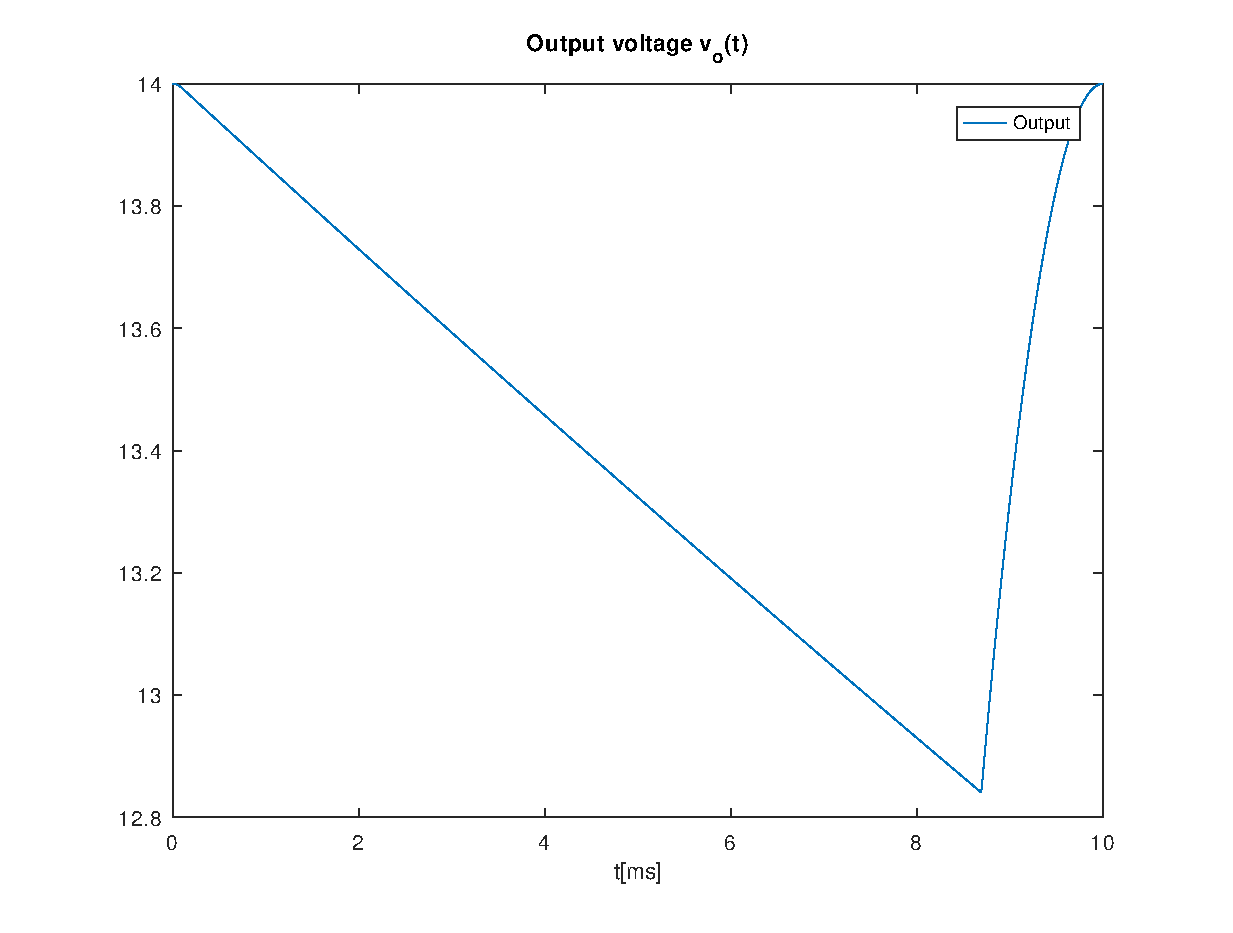
\includegraphics[width=0.6\textwidth]{envelope.eps}
\caption{The final envelope detector circuit voltage $v_0$ during a half-period interval.}
\label{fig:envelope}
\end{figure}

where $t$ is expressed in miliseconds (ms) along the x-axis\\
and $v_0$, the envelope output voltage, is expressed in Volts (V) along the y-axis.
%%%%%%%%%%%%%%%%%%%%%%%%%%%%%%%%%%%%%%%%%%%%%%%%%%%%%%%%%%%%%%%%%%%%%%%%%%%%%%%%%%%%

\subsection{Voltage Regulator Circuit}
\label{subsec:regulator}

\paragraph{}
The voltage regulator attenuates oscillations in the input signal without frequency dependence and takes advantage of the non-linear characteristic of the $N$ diodes included in the positive voltage limiter. 

We start by defining some of the parameters needed in the composition of a voltage regulator circuit, suchs as the resistor $R_2$ value and the number of diodes $n$ of the voltage limiter. We also present the diode's characteristic values, such as the emission coefficient $\eta$, the reverse saturation current $I_S$, the thermical voltage $v_T$ and the diode voltage $v_D$.

\[
\left\{\begin{matrix}
N=17\\
R_2=10k\Omega=10 000\Omega\\
\eta=1\\
v_t=0.025 V\\
v_d=0.706 V\\
I_s=1\times10^(-14)\\
\end{matrix}\right.
\]


The voltage analysis of the regulator applies the incremental analysis method, separating the DC and incremental components.

\paragraph{}
The diode incremental resistance is calculated using the following expression: $r_d=\frac{\eta v_t}{I_s e^(\frac{v_d}{\eta v_t}}$.

Applying the voltage divider rule, the AC increment $v_{out}$ is defined using the following relation: $vout=\frac{N r_d}{N rd+R2}vO$.

It is easy to understand that a large value of the resistor $R_2$ will maximize the denominator and make it significantly bigger than the numerator ($N rd+R2 >> N r_d$), which makes the whole quotient tend to zero ($\frac{N r_d}{N rd+R2} \longrightarrow 0$). While we minimize the AC increment, we are at the same time increasing the precision of the DC voltage, as pretended when building an AC-DC converter.

\paragraph{}
On the other hand, the DC voltage $V_{OUT}$ is obtained multypling the diode voltage $v_d$ by the number of diodes $N$ used in the voltage regulator circuit: $V_{OUT}=N v_d$.

\paragraph{}
The final voltage of the regulator circuit $v_{OUT}$ is obtained adding the results of the incremental analysis and the DC analysis: $v_{OUT}=v_{out}+V_{OUT}$.

\begin{figure}[H] \centering
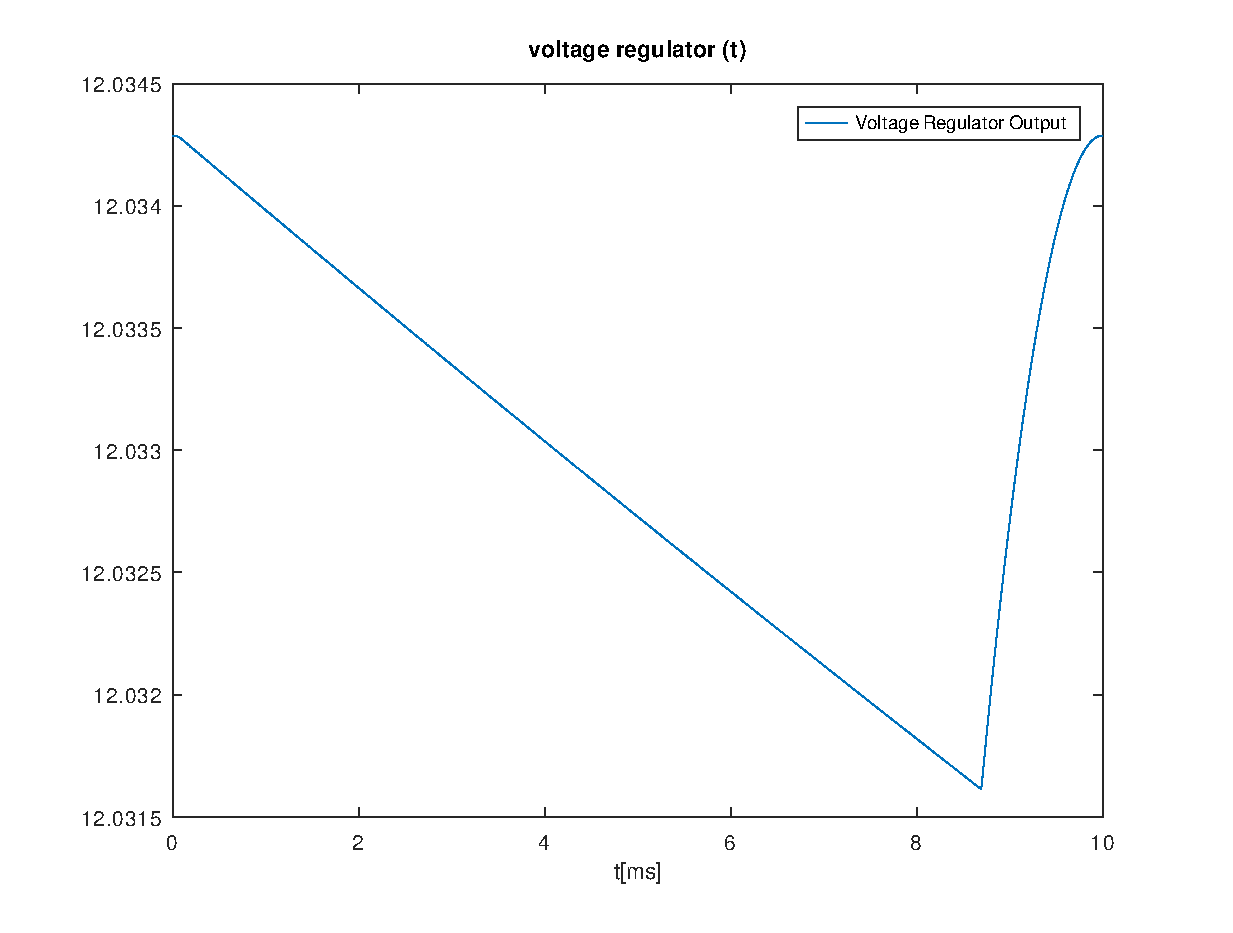
\includegraphics[width=0.6\textwidth]{output.eps}
\caption{The final voltage $v_{OUT}$ of the voltage regulator circuit during a half-period interval.}
\label{fig:output}
\end{figure}

where $t$ is expressed in miliseconds (ms) along the x-axis\\
and $v_{OUT}$, the voltage of the regulator, is expressed in Volts (V) along the y-axis.
%%%%%%%%%%%%%%%%%%%%%%%%%%%%%%%%%%%%%%%%%%%%%%%%%%%%%%%%%%%%%%%%%%%%%%%%%%%%%%%%%%%%%

\subsection{Voltage Ripple}
\label{subsec:ripple}

\paragraph{}
The voltage ripple can be improved using a full-wave rectifier circuit in the envelope detector circuit. 

The value of the voltage ripple $v_{ripple}$ can be calculated relating the maximum and the minimum values of the final voltage of the regulator circuit $v_{OUT}$, using the following expression: $v_{ripple}=max(v_{OUT})-min(v_{OUT})$.

\begin{center}
   \begin{tabular}{|c||c|}
      \hline
        
 The Output Voltage RIPPLE is & 0.00238568 V \\ \hline 
   \end{tabular}
 \end{center}

%%%%%%%%%%%%%%%%%%%%%%%%%%%%%%%%%%%%%%%%%%%%%%%%%%%%%%%%%%%%%%%%%%%%%%%%%%%%%%%%%%%%%
\subsection{The Output DC Level}
\label{subsec:dclevel}

\paragraph{}
The $t_{ON}$ is calculated using the Newton-Raphson iterative method, starting with a function obtained through the following equation: $Acos(\omega t_{ON})=Acos(\omega t_{OFF})e^(\frac{-(t_{ON}-t_{OFF})}{RC})$.

The DC level output average is obtained integrating the sinusoidal and exponential functions during a half-period interval. The calculations are shown below.\\

$t\in[0,t_{OFF})]\\
\int_{0}^{t_{OFF}}=\frac{N r_d}{N r_d + R_2}\frac{A}{\omega}sin(\omega t_{OFF})+N v_d t_{OFF}\\$\\

$t\in[t_{OFF},t_{ON}]\\
\int_{t_{OFF}}^{t_{ON}}=\frac{N r_d}{N r_d + R_2}(-A R C cos(\omega t_{OFF})(e^{\frac{-({tON}-{tOFF})}{RC}}-1))+N v_d (t_{ON} - t_{OFF})\\$\\

$t\in[t_{ON},\frac{T}{2}]\\
\int_{t_{ON}}^{\frac{T}{2}}=\frac{N r_d}{N r_d + R_2}\frac{A}{\omega}(sin(\omega \frac{T}{2})-sin(\omega t_{ON}))+N v_d (\frac{T}{2}-t_{ON})\\$\\

$\overline{V}=\frac{\int_{0}^{t_{OFF}}+\int_{t_{OFF}}^{t_{ON}}+\int_{t_{ON}}^{\frac{T}{2}}}{\frac{T}{2}}$

\begin{center}
   \begin{tabular}{|c||c|}
      \hline
        
 THE OUTPUT VOLTAGE AVERAGE LEVEL IS & 12.0248 V \\ \hline 
   \end{tabular}
 \end{center}

The Output DC Level accuracy can be evaluated through comparing the final voltage of the circuit $v_{OUT}$ and the $12 V$ constant function. 

\begin{figure}[H] \centering
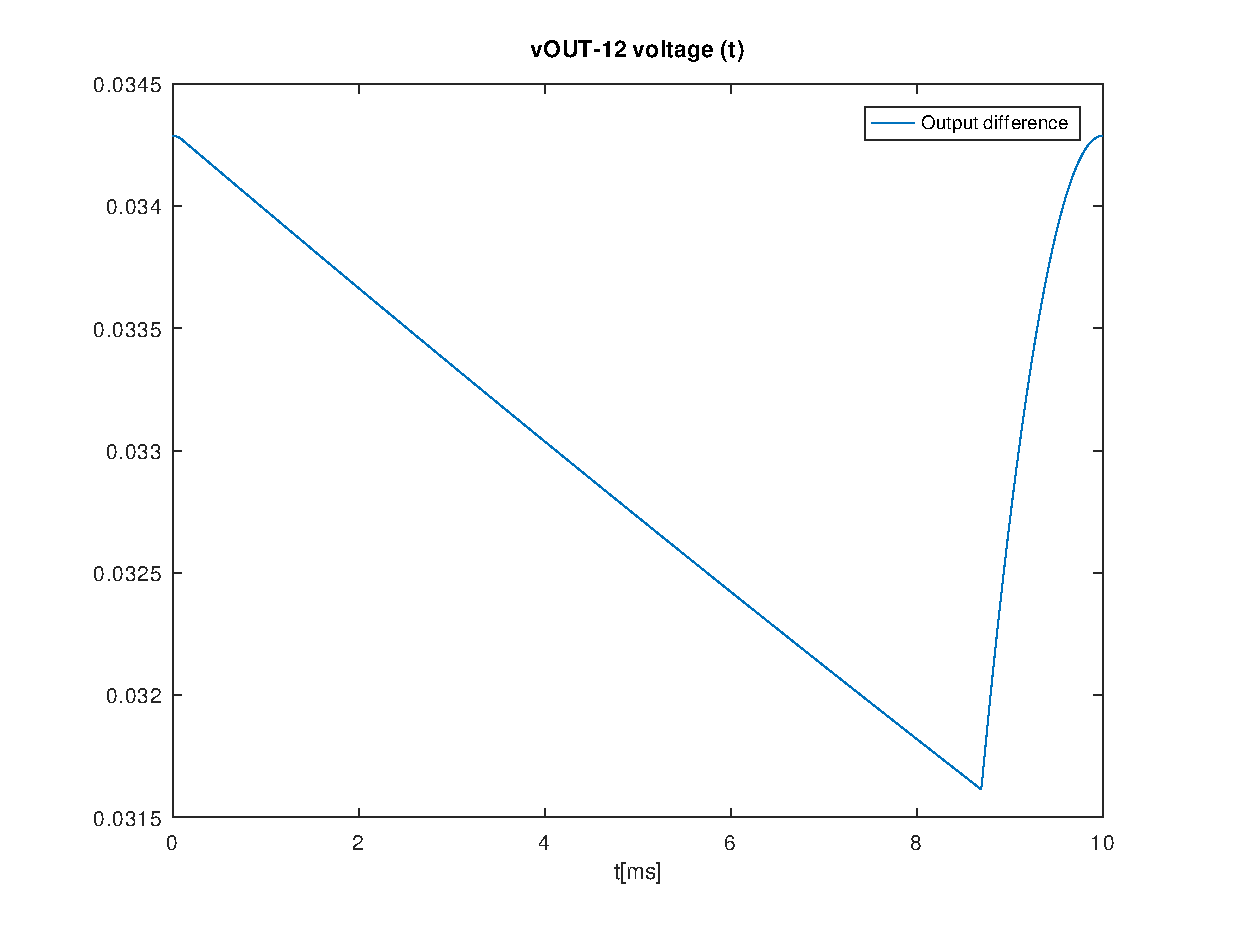
\includegraphics[width=0.6\textwidth]{outputdiff.eps}
\caption{The voltage $(v_{OUT}-12)$ during a half-period interval.}
\label{fig:outputdiff}
\end{figure}

where $t$ is expressed in seconds (s) along the x-axis\\
and $(v_{OUT}-12)$, the output voltage difference, is expressed in Volts (V) along the y-axis.
